\documentclass[msc,pdftex]{coppe}
%other options
%doublespacing HAHHAHAHAHAH

% VEJA SE ISTO ATRAPALHA OU AJUDA
% PRECISAMOS DE UM PACOTE PARA EU COMENTAR
\usepackage[show]{ed}
\def\ednoteshape{\color{red}}
% esse gerou muitos erros
%http://repositorios.cpai.unb.br/ctan/macros/latex/contrib/ed/ed.pdf
%\usepackage{todonotes}
%http://www.lasca.ic.unicamp.br/pub/ctan/macros/latex/contrib/todonotes/todonotes.pdf

\usepackage{enumitem}
\usepackage{multicol}
\usepackage[T1]{fontenc}
\usepackage[utf8x]{inputenc}
\PrerenderUnicode{ě} %for bibitem beholavek2002
%\usepackage[brazil]{babel}
\usepackage{verbatim}
\setcounter{secnumdepth}{4} %numbering subsubsections
\setcounter{tocdepth}{4} %subsubsections in table of contents
\usepackage[ruled,vlined,linesnumbered]{algorithm2e}
%portuguese
\usepackage{amsmath,amssymb}
\usepackage{relsize}
\usepackage{graphicx}
\usepackage{courier}

% definitions
\usepackage{amsthm}
\theoremstyle{definition}
\newtheorem*{definition}{Definition}

%subcaption and subfigure
%\usepackage{subfig}
\usepackage{caption}
\usepackage[labelformat=simple]{subcaption}
\renewcommand\thesubfigure{ (\alph{subfigure})}

%apud citation style
\newcommand{\apudp}[2]{(\citeauthor{#1},\space\citeyear{#1},\space as cited in \citeauthor{#2},\space\citeyear{#2})}
\newcommand{\apud}[2]{\citeauthor{#1}\space (as cited in \citeauthor{#2},\space\citeyear{#2})}

%full centered cell
\newcommand{\specialcell}[2][c]{%
  \begin{tabular}[#1]{@{}c@{}}#2\end{tabular}}
\usepackage{multirow}
%\usepackage{array}

\usepackage[hyphens]{url}
\usepackage{hyperref}
\usepackage{lmodern}
\usepackage{rotating}
\usepackage{tikz}
\usepackage{pgfplots}
\usepackage{ucs}

\usepackage{lipsum}

\usepgflibrary{fpu}
\usetikzlibrary{shapes.multipart, mindmap, arrows}

%preventing widow and orphan lines
\widowpenalty=10000
\clubpenalty=10000
\postdisplaypenalty=10000

%footnote in verty bottom
\usepackage[bottom]{footmisc}

\usepackage{float}
\usepackage{todonotes}

\makelosymbols
\makeloabbreviations

\pgfplotsset{compat=1.12}

\begin{document}
	\title{Social Tag Prediction: A Resource-centered Approach for Broad Folksonomies}
	\foreigntitle{Predição de Rótulos Sociais: Uma Abordagem Baseada em Recursos para Folksonomias Largas}
	\author{Felipe de Queiroz Badejo}{Almeida}
	\advisor{Prof.}{Geraldo Bonorino}{Xexéo}{D.Sc.}
	\advisor{Prof.}{Fellipe Ribeiro}{Duarte}{D.Sc.}
	%\advisor{Prof.}{Nome do Terceiro Orientador}{Sobrenome}{D.Sc.}
	
	\examiner{Prof.}{Geraldo Bonorino Xexéo}{D.Sc.}
	\examiner{Prof.}{Jano Moreira de Souza}{Ph.D.}
	\examiner{Prof\textordfeminine.}{Renata Mendes de Araújo}{D.Sc.}
	%\examiner{Prof.}{Nome do Quarto Examinador Sobrenome}{Ph.D.}
	%\examiner{Prof.}{Nome do Quinto Examinador Sobrenome}{Ph.D.}
	\department{PESC}
	\date{03}{2018}
	
	\keyword{social tagging systems}
	\keyword{multi-label classification}
	\keyword{multi-label ranking}
	\keyword{tag prediction}
	\keyword{tag recommendation}
	\keyword{text classification}
	
	\maketitle
	
	\frontmatter
	\dedication{To my family.}
	\chapter*{Acknowledgments}



\ednote{TODO}
	\begin{abstract}
Este trabalho apresenta um novo método para a predição de rótulos (tags) associadas a objetos em um ambiente colaborativo de atribuição de tags (comumente chamados de \textit{Social Tagging Systems}), onde estes objetos são tagueados por membros da comunidade de forma livre. Experimentos são realizados em dois conjuntos de dados e os resultados obtidos são relatados.
\end{abstract}
	\begin{foreignabstract}
\ednote{todo}
\end{foreignabstract}
	\tableofcontents
	\listoffigures
	\listoftables
	\printlosymbols
	\printloabbreviations
	
	\mainmatter
	\chapter{Introduction}\label{chap:intro}

{\color{red} TODO: talk about the explosion in Internet usage, say that it is getting ever harder to categorize stuff, mention that examples of STS will be given in the next sections.

say that we will use "social tagging systems" and "folksonomies" interchangeably. }

\section{Motivation}\label{section:intro_motivation}

The motivation for this work is twofold. 

Firstly, I myself take part in many online communities, including some where I need to organize resources in one way or another. I am frequently frustrated with the fact that many websites do not provide any organization capabilities other than placing things in \textit{categories} or \textit{folders}.

I am witness to the fact that these methods don't scale at all for anything other than trivial examples \footnote{Say you need to place a scientific article called \textit{The History of Football in Europe} in a folder. Do you place it under "history", "sports" or under "Europe"?} and I believe tagging is a good way forward.

Secondly, it is well established that suggesting tags to users promotes faster convergence to a common vocabulary \citep{marlow_etal_2006,hassan_etal_2009, dattolo_etal_2010} and increases the likelihood that resources are tagged \citep{dattolo_etal_2010,floeck_etal_2010}. Additionally, it has been claimed that identifying good tags from a set of recommended tags is orders of magnitude less demanding than coming up with good tags without intervention \citep{marinho_etal_2012}.

Since there is massive amounts of data available from Social Tagging Systems (STSs), it's natural to think of a data-driven, machine-learning based method to pursue that goal. We realized that predicting tags for resources in a social setting would not only be a worthy problem from a theoretical standpoint, but could also effectively help people in the real world navigate these online communities.

\section{Problem scope}\label{section:intro_problem}

When considering Social Tagging Systems, one can envision many different problems and areas where scientific knowledge and research could be put to use.

We chose to address the problem of how to correctly predict which tags will be used to describe a given textual object in such a system. 

Since this problem touches upon many areas of scientific knowledge, such as machine learning, natural language processing (for textual resources), computer vision (similarly, for images and visual objects), recommender systems and so on, we would like to further limit our scope in a more precise manner.

Firstly, one may create a distinction (according to commonly-cited sources such as \cite{wal_2005_broad_and_narrow}) between \textbf{broad} and \textbf{narrow folksonomies}. Broad folksonomies are those where not just a resource's owner but the whole community of users may assign tags to any one resource available on the system. Narrow folksonomies, on the other hand, only allow items to be tagged once, by the person who has first added that particular item to the system (i.e. that item's owner).

Broad folksonomies exhibit more diversity and richness of information, not to mention sheer scale, which makes them more amenable to analysis by data-driven methods, such as machine learning. More concretely, it has been suggested that a shared, global vocabulary of tags cannot be observed in narrow folksonomies \citep{schifanella_etal_2010}.

Secondly, many authors \citep{illig_etal_2011,song_etal_2011} have made a distinction between \textbf{resource-centered} and \textbf{user-centered approaches}. This refers to the fact that some approaches take user information into account when performing tag prediction (user-centered) while others take a global view, giving the same predictions for every user (resource-centered).\footnote{Other authors, e.g. \cite{zhang_etal_2014} refer to these two types as \textit{personalized} and \textit{collective} tag recommendation.}

We have chosen to focus on resource-centered approaches to predicting tags in broad folksonomies. This is due to the previous reasons and to the fact \citep{song_etal_2011} that user-centered approaches do not perform so well vis-a-vis resource-centered methods; the distribution of users and tags in broad folksonomies follow a power law and reusability of tags by each individual user is low. 

This makes resource-centered approaches more robust as we generally have much more information about resources than about users. This is particularly true with textual resources and broad folksonomies. Also, resource-centered methods have the added benefit of being able to work in the absence of user information, the so called \textit{cold start} problem.

Additionally, we would like to point out that most similar works in the literature do not take into account the number of times each tag has been assigned to a given resource. In other words, a \textit{binary} tag-assignment model or \textbf{BTAS} \citep{illig_etal_2011} is used, whereby a tag assignment is equated with the fact that \textit{there exists at least one} user who assigned that tag to that resource. We follow that convention in this article.

\begin{definition}{BTAS}\footnote{Adapted from \cite{illig_etal_2011}.}

Let $TAS$ be all tag assignments made by all users $u \in U$, using tags $t \in T$ for resources $r \in R$:
\[ TAS = \{ (u,t,r) \in  U \times T \times R \ | \ \text{user} \ u \ \text{has assigned tag} \ t \ \text{to resource} \ r \} \]  

$\mathbf{BTAS}$ abstracts the user dimension away, considering instead a \textit{binary} tag assignment $(t,r)$ the existence of \textit{any} user $u$ having assigned tag $t$ to resource $r$:

\[ BTAS = \{(t,r) \in T \times R \ | \ \exists u \in U : (u,t,r) \in TAS \}  \]

\end{definition}

More information on these issues is given in \autoref{chap:social_tagging}.

\section{Methodology}\label{section:intro_methodology}

Here we will give a brief overview of the research methodology used in this work.

\subsection{Systematic Literature Review}\label{section:literature_review}

In order to add replicability and transparency to our literature review, we adopted principles from Systematic Literature Review, as defined in works such as \cite{baumeister_leary_1997} and \cite{bem_1995}.\footnote{Evidence such as screenshots of search results and the actual set of articles retrieved from each query can be provided upon request.}

We selected three reputable repositories of scientific articles and research pieces, namely IEEE-XPlore Digital Library\footnote{http://ieeexplore.ieee.org/Xplore/home.jsp}, ScienceDirect\footnote{https://www.sciencedirect.com/} and Scopus\footnote{https://www.scopus.com/}.

After initial contact with the subject matter of our work, we selected four sets of search terms, namely \textit{"collaborative tagging"}, \textit{"social tag prediction"}, \textit{"social tagging"} and \textit{"tag prediction"} and used those to search the titles, abstracts and contents of research pieces in the websites' databases.\footnote{These search terms were chosen because we believe they encompass a large part  of the available literature related to the topic of our work which we defined (for the purpose of this literature review) as \textbf{"Predicting or recommending tags in a social tagging environment"}.} 

We gathered and organized the results of the aforementioned queries; after removing duplicated entries, we had a collection of 2466 articles, book chapters or conference proceedings.

We read the abstracts of all 2466 pieces and, based on that, we selected 399 as being somehow related to the subject of our work, as explained above.

Out of these 399 relevant works, we further refined our set to 285 articles, by extending our analysis to the introduction and conclusion sections. This final list of 285 articles all contained information directly related to the task of predicting and/or recommending tags in a social tagging environment. They were all read in order to inform our research.\footnote{Other articles, which didn't feature in the search results, but were obviously relevant (based upon citation count for example), were also added and read.}


\section{Document structure}\label{section:intro_structure}

{\color{red} TODO: do this when the chapters are finished.}

{\color{red} TODO: add final sections and section numbers here In \autoref{chap:intro} \ldots Finally, \autoref{chap: conclusion} we conclude and point to possible ways in which this work may be extended and/or continued.}




	\chapter{Social Tagging}\label{chap:social_tagging}

The massive expansion experienced by the Internet and web communities in the last decades has undoubtedly had a large effect on how we live our lives.

Today, we have access to many kinds of services on the web, such as search engines, email messaging, online purchases, and so on.

However, some of the most widely used websites are places where people interact with digital resources and with other human beings. Among these we could cite websites such as Facebook, Twitter, Youtube, StackOverflow, Quora, LinkedIn, Reddit, Sina Weibo and many others.

These online communities form what is commonly referred to \textit{social media} or \textit{social networking services}, or SNSs. \citep{obar_wildman_2015,hamburger_etal_2017}

Moreover, some of these so-called social media services support \textit{tags}, which are user-given, generally free-form, keywords used to help categorize resources \cite{mathes_2004}. These systems are called \textbf{Social Tagging Systems} or \textbf{STS}s.

We will go into more detail about these concepts, as well as some related terms (such as folksonomies) in the next sections.

\section{Examples of Social Tagging Systems}

Examples of STSs abound in the modern Web. We will present two different examples so that the reader can better grasp what a Social Tagging System looks like in practice.

\subsection{MovieLens}

MovieLens \footnote{https://movielens.org} is a research website run by GroupLens Research at the University of Minessota.

It provides users with personalized movie recommendations based on how they have rated individual films. In addition to information and ratings for many movies, MovieLens also lets users add tags to movies and view tags others have assigned.

As can be seen in the following image, tags allow users to give objective (\textit{car chase, espionage}) and subjective (\textit{great plot} attributes to resources, in this case films.

\begin{figure}[H]
    \centering
    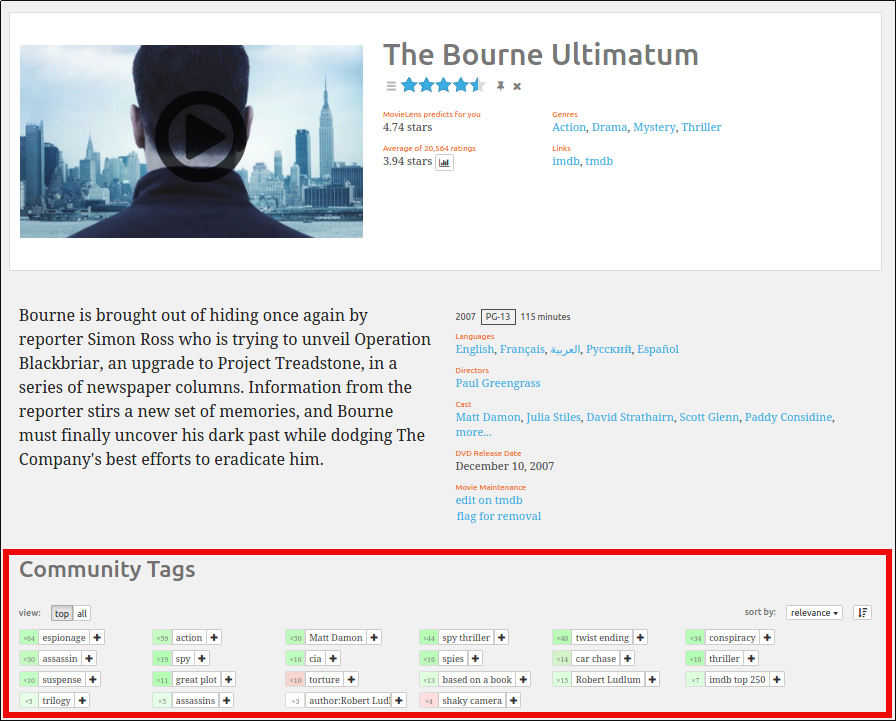
\includegraphics[width=\textwidth]{chapters/02_social_tagging/images/movielens.png}
    \caption{The MovieLens website supports tagging; any user can add their own tags and view tags assigned by other users to a particular resource. Retrieved from https://movielens.org/movies/54286 in January 2018.}
    \label{fig:movielens}
\end{figure}

\subsection{StackOverflow}

StackOverflow \footnote{https://stackoverflow.com/} is a very popular Q\&A (Question and Answer) website. It receives roughly 8,000 new questions related to computer programming every day. \footnote{As of 2017: https://stackoverflow.blog/2017/05/09/introducing-stack-overflow-trends/}

StackOverflow supports tagging of questions; users can add up to 5 tags to every question they post. Among other features, tags can be used to narrow down search results and they can also be subscribed to. Tags are also part of the website's incentive and reputation mechanisms; you can be awarded \textit{tag medals} for completing specific objectives such as answer many questions having a particular tag.

\begin{figure}[H]
    \centering
    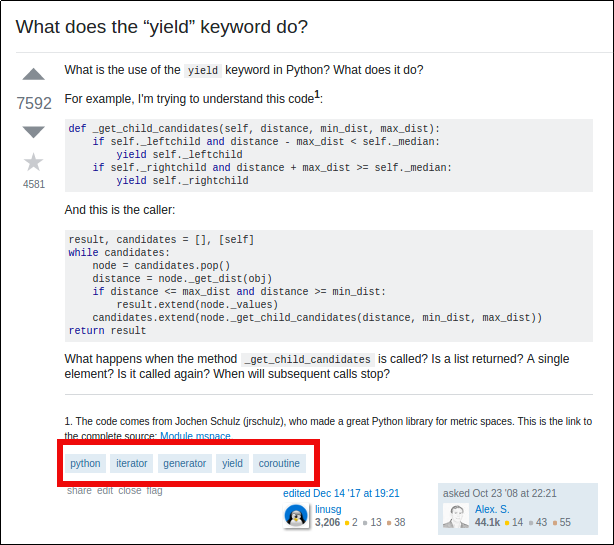
\includegraphics[width=\textwidth]{chapters/02_social_tagging/images/stackoverflow.png}
    \caption{The StackOverflow website also supports tagging, but only a single set of tags is shown, namely the tags assigned by the resource's original owner (and maybe edited afterwards). Retrieved from https://stackoverflow.com/questions/231767/what-does-the-yield-keyword-do in January 2018. }
    \label{fig:stackoverflow}
\end{figure}

\begin{figure}[H]
    \centering
    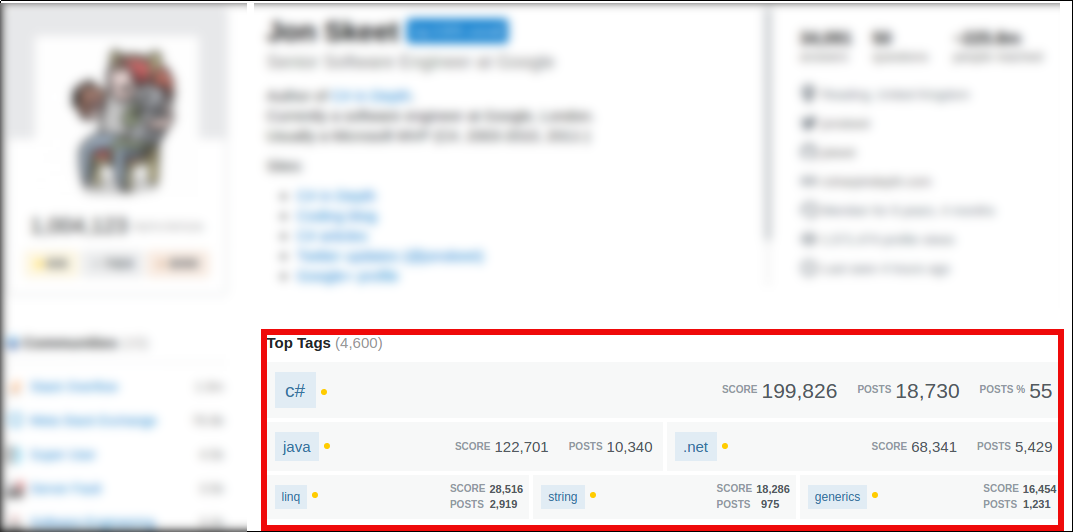
\includegraphics[width=\textwidth]{chapters/02_social_tagging/images/jon_skeet.png}
    \caption{Tags are also used to help drive Stackoverflow's incentive mechanisms; tag medals are awarded for activity related to a certain tag. Retrieved in January 2018. (Blur is used to protect the user's privacy)}
    \label{fig:jon_skeet}
\end{figure}

\section{Social Tagging and Folksonomies}

Since the beginning of STSs, it has been observed that such systems grow in an organic way and that certain patterns are noticed with respect to how tags are used. As an example, it has been observed \citep{halpin_etal_2006} that the number of times each tag is used to tag a particular resource forms a \textit{power law}, i.e. some tags are used exponentially more often than others.

More generally, the term \textbf{folksonomy} has been used to describe  these emerging patterns of informal organization and meaning assumed by tags in a Social Tagging System \citep{mathes_2004,wal_2005_folksonomy}.

{\color{red} TODO: ADD here mathematical formulation of folksonomies (tripartite graph model) as per \cite{mika_2007}}

The word \textit{folksonomy} itself (formed by \textit{folk} + \textit{taxonomy}) points to the fact that, differently from a rigid, often expert-driven taxonomy, the patterns that arise with the free use of tags by a community follows a more fluid, hapzard fashion, as can be  visualized in the next image where the the tag \textit{afghanistan} was used as search criterium on a photo-sharing website: 

\begin{figure}[H]
    \centering
    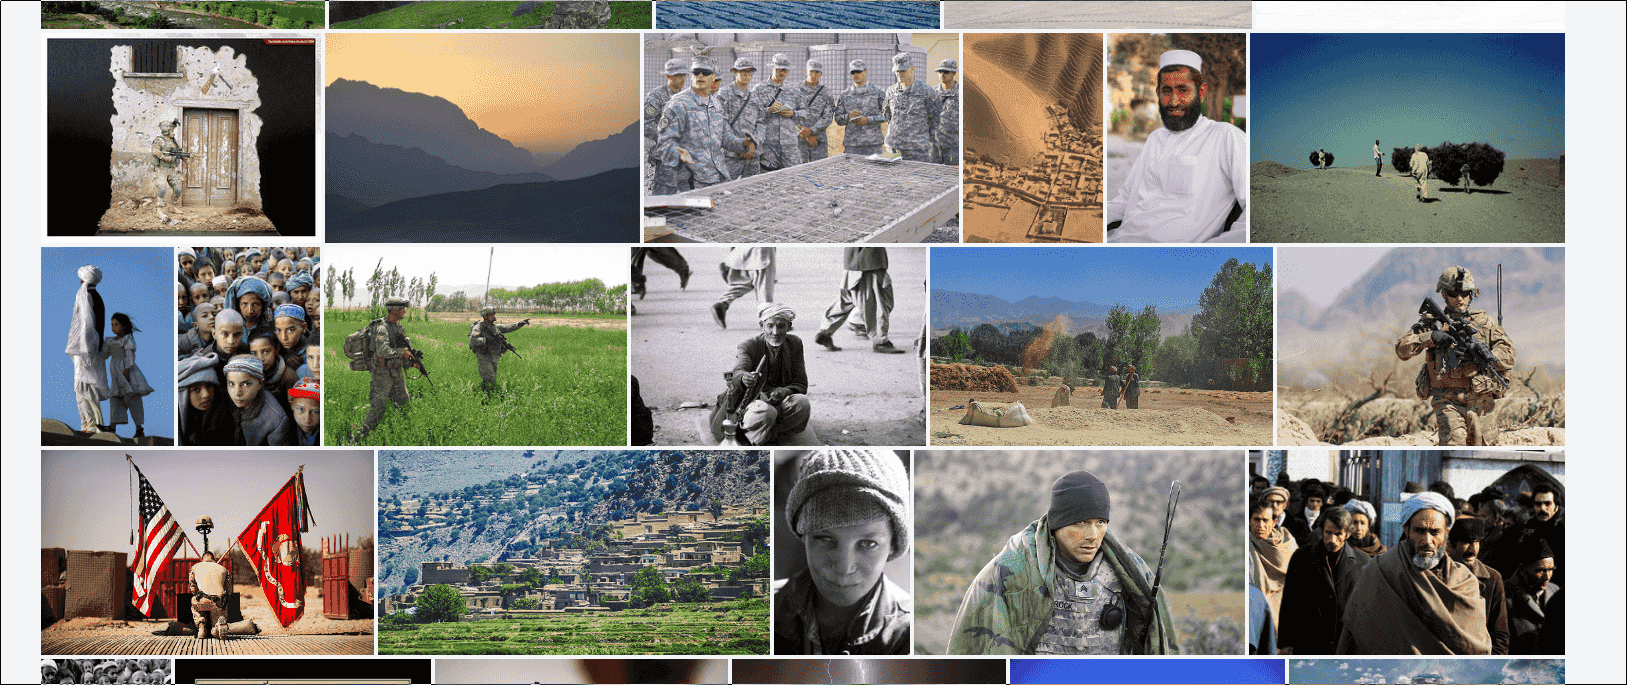
\includegraphics[width=\textwidth]{chapters/02_social_tagging/images/flickr_afghanistan.png}
    \caption{Searching for images tagged \textit{afghanistan} on Flickr yields pictures from the Afghani people, the war in Afghanistan, the Afghani landscape, etc. This reflects the multitude of meanings a single tag may acquire due to the way users tag their pictures. Retrieved from https://www.flickr.com/search/?tags=afghanistan in January 2018.}
    \label{fig:afghanistan}
\end{figure}

\section{Narrow and Broad Folksonomies}

Based on the examples given and one's general day-to-day experience, it's natural to conclude that folksonomies and their underlying STSs vary widely with respect to their features and how they're implemented.

One basic difference, raised as early as 2005 \citep{wal_2005_broad_and_narrow} and commented on by other authors \citep{marlow_etal_2006,halpin_etal_2006,peters_2009} since, is that between \textit{narrow} and \textit{broad} folksonomies.

\textbf{Narrow} folksonomies are folksonomies which only allow a resource's original poster (commonly referred to as \textit{O.P.} in such systems) to add tags to that resource. In other words, \textit{users can only tag their own content}.

Conversely, \textbf{broad} folksonomies are those where every user can add tags to any resource on the platform.

This distinction is relevant for researchers studying the dynamics of social tagging systems. For example, it has been noted by \cite{schifanella_etal_2010} that a global, shared tag vocabulary cannot be observed in narrow folksonomies, unless it is specifically promoted by the system.

On a similar note, \cite{aiello_2012} have suggested that tag predicting is more meaningful in broad folksonomies, since users can tag the same, global, set of resources. Also, tagging in such systems tend to reflect resource contents rather than users' personal preferences.

As related to the ease of navigation in STSs, \cite{helic_etal_2012} have suggested that broad folksonomies are better and more efficient for user browsing, inasmuch as these tags encode more information than their counterparts in narrow systems.

\section{Other Aspects}

Here we will talk about a few other aspects which we deem relevant in light of this work's objective, namely that of predicting tags in STSs.

\subsection{Tag Stabilization and Convergence}

In broad folksonomies (i.e. those where all users can add tags to any resource), the tag distribution for a given resource has been observed to stabilize after about 100 individual tag assignments \citep{golder_huberman_2006}. Reasons given for this phenomenon include \textit{imitation}, i.e. users are influenced by other tags already given to a resource and \textit{shared knowledge}, i.e. other tags help build a user's mental model of the meaning for each tag.

We consider this an important result because it may affect the level of tag prediction we can achieve. One can view it graphically in the following image:

\begin{figure}[H]
    \centering
    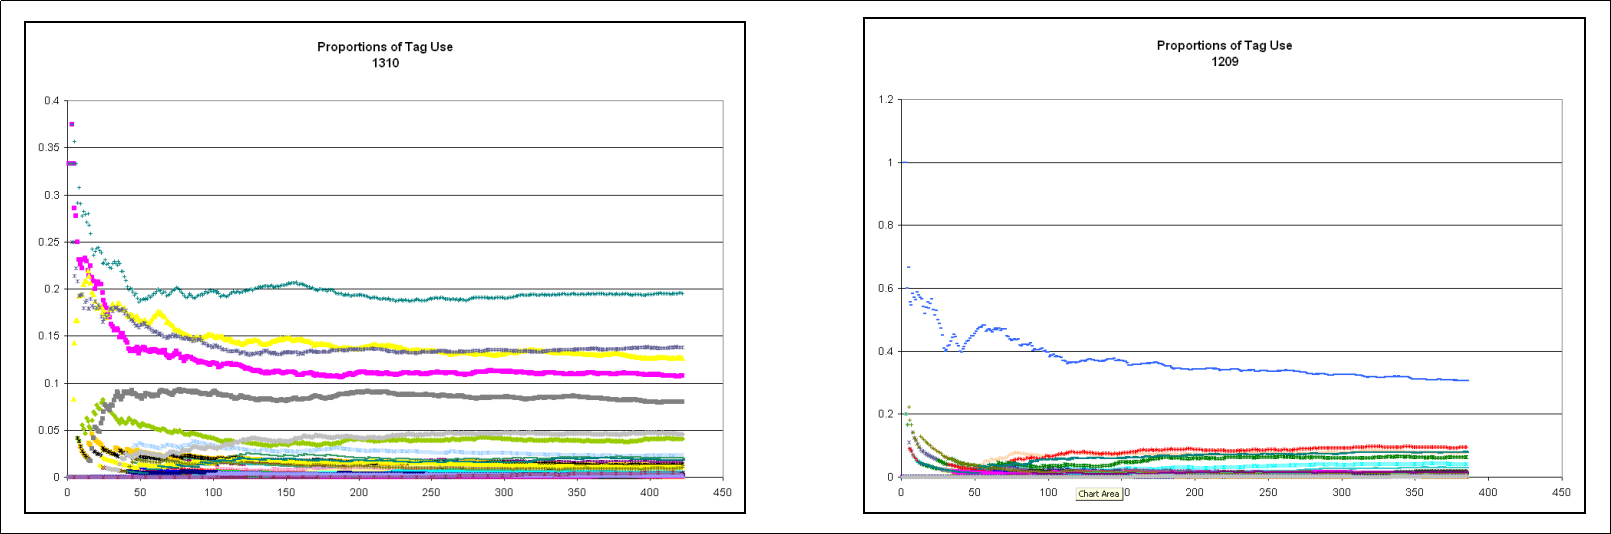
\includegraphics[width=\textwidth]{chapters/02_social_tagging/images/golder_huberman.png}
    \caption{Tag distributions for two resources on Delicious.com. Tag proportions reach equilibrium after around 100 tag assignments. Adapted from \cite{golder_huberman_2005}}
    \label{fig:golder_huberman}
\end{figure}

\subsection{Effect of tag suggestion on STSs}

It has been suggested by \cite{marlow_etal_2006} that a STS falls under one of three types depending upon how much system support there is for tagging:

\begin{itemize}[noitemsep]
\item \textit{Blind Tagging}: Users cannot view other tags assigned to an item, before adding their own.
\item \textit{Viewable Tagging}: Users can view other tags assigned to an item before adding their own tags.
\item \textit{Suggestive Tagging}: Users can not only view other tags but the system also suggests appropriate tags.\citep{marlow_etal_2006}
\end{itemize}

They have suggested that the level of tagging support (as referred to above) present in a system may make tag stabilization and convergence faster.

In light of that, we can suggest that tag prediction can contribute to a higher quality STS, if we assume that a folksonomy where the global vocabulary has converged is more useful than one where it hasn't.



	\chapter{Related Work}\label{chap:related_work}

In this section, we will present general approaches to tag prediction, with a special focus on resource-based methods for broad folksonomies, that being our problem scope.

\section{Introduction}

{\color{red} TODO: short intro here, talk about resource-centered, user-centered, cite ties to recommender systems, multi label classification and multi label ranking.}

As related to how authors name their particular approaches, one should be careful inasmuch as there is no apparent consensus as to what constitutes a \textit{recommendation} approach vis-a-vis a \textit{prediction} approach with respect to STSs. 

It is frequently the case in the literature that the word "recommendation" is used to refer to methods that use no user-specific information whatsoever and, conversely, words like "prediction" and "suggestion" used in cases where personalized recommendations are made.

\section{Resource-centered Methods}\label{section:resource_centered_methods}

In this section, we present a collection of  \textit{resource-centered} methods for tag prediction. They are so called because they leverage only resource-specific information in order to predict what tags should be assigned to a new, unlabelled resource. In other words, all prediction are of \textit{unpersonalized} nature.

We note that, although our problem domain only includes textual documents, we chose to also mention in this section approaches used in other domains, such as audio, video and images. This is because we are mostly interested in how these approaches work irrespective of the choice of features used.

\subsection{Association Rule Mining}

{\color{red} TODO: introduction to association rule mining}

In one of the earlier papers on social tag prediction, HEYMANN et al. \citeyearpar{heymann_etal_2008} have applied \textit{association rules} of the form $X \rightarrow Y$ (where $X$ and $Y$ are tagsets) in order to expand the set of tags given to a resource. Using techniques such as \textit{Market Basket Analysis}, the authors derive association rules of length 4 and below, using a certain level of support\footnote{A rule's \textit{support} equals the number of examples where both $X$ and $Y$ are present.} as threshold to remove overly noisy rules.

The authors report \citep{heymann_etal_2008} that a surprisingly high number of high quality rules can be found (such as those representing \textit{type-of} relationships and synonyms). Furthermore, the added tags help increase precision and recall for user queries, when the result sets are augmented to include documents tagged with those tags.

The authors also claim that using larger and larger rules would probably increase performance, but computational complexity quickly become prohibitive.\footnote{Note that this method assumes that a resource already has some tags assigned to it. These are then used to predict another set of tags. This is sometimes called \textbf{tag-set expansion} in order to differentiate it from methods that do not make this assumption.}

Another approach involving association rules was put forward by \cite{vanleeuwen_puspitaningrum_2012}. They acknowledge the fact that gains in performance brought about by using larger rules come at a high cost in terms of processing time. They, however, suggest that a compromise can be achieved by choosing a carefully selected set of association rules, such that performance is increased at a lower cost.

Their approach works by using a compression mechanism to efficiently compute expanded tagsets for any given tagset. It computes the most suitable expanded tagsets ranked by support.\footnote{The support for a given tagset is simply the number of times that particular tagset was assigned to a resource in the system.}

\subsection{Content-based tag propagation}

Here we provide a basic overview of methods which, in one way or another, use the content-based similarity to propagate tags from labelled instances to unlabelled ones.

In the first approach, \cite{sordo_etal_2007} have used both first-order (stylistic) and second-order (mood-based, extracted from the stylistic ones) features and a neighbours-based similarity measure to propagate labels from labelled audio pieces to unlabelled ones.

They reported good results for the approach, as measured by rank-based metrics such as Spearman's rank and Precision@$k$. They claim that ignoring tags with too few assignments improves results and that sometimes using more neighbors is beneficial, while sometimes it's harmful.

It should be noted here that this work was not run on a broad folksonomy, since all examples were annotated by a single person.

Another interesting example is that of \cite{moxley_etal_2008}. Their approach uses many feature \textit{modalities} to represent a resource (in this case, videos). In other words, they use multiple sources of information to build a feature vector, namely text information from the video transcripts, image information from video snapshots and concept information from external source.

They report good results using set-based performance metrics (slight variants of precision and recall). Furthermore, they claim that using an average of features built from multiple modalities helps suppress the effect of noisy information.

In \cite{guillaumin_etal_2009}, the authors propose a weighted neighbor approach where one can choose an arbitrary distance measure (i.e. Euclidean, Manhattan, etc) one wishes to use to measure similarity between resource representations. Then, the optimal weights for each resource are found via the optimization of a custom loss function that encodes the accuracy each individual tag prediction. 

In other words, the dataset is used to inform the decision on what weights to use for each resource. This will, in turn, define to what extent tag assignments for each resource will influence those of its neighbors.

This approach has been called \textit{metric learning} and, according to the authors, it has been used in the past in other contexts.

In \cite{li_etal_2009}, the authors have approached the problem from a slightly different angle. Although they have also used content-based similarity to search for neighbors, the weight given to each tag is not just proportional to the similarity between each pair of neighbors; it also incorporates a term that normalizes each tag according to the tag's \textit{prior}, i.e. the overall frequency of a given tag in the whole dataset.

By using rank-based metrics such as Precision@$k$ and Mean Average Precision (MAP), they report that their method consistently outperforms approaches that do not take a tag's overall prior into account.

In conclusion, two common themes in such \textit{content-based} tag propagation approaches seem to be \textbf{a)} designing similarity measures and other ways to retrieve similar resources given a query resource and \textbf{b)} once the neighbor resources are found, find meaningful ways to weigh the contribution given by each neighbor in order to predict tags for the query resource. 

\subsection{Resource-based tag propagation}

In this subsection, we will talk about methods which use information \textit{about} the resource (other than its contents encoded as features) to build representations for these resources. These representations are then used in neighbor-based algorithms for actual classification.

{\color{red} TODO: can I find some OTHER guy who just represented each resource as a vector over tags and did something simple with it?}

\cite{auyeung_etal_2009} propose a slightly different approach. They encode each resource as a vector over the space of the full tag vocabulary, so that it resembles a bag-of-words approach, using tags instead of terms in the document. Similarity between resources is then calculated via simple measures like cosine similarity.

The authors report above-benchmark performance when using the described approach to predict tags for unlabelled examples. Metrics used to for gauging performance include Precision@$k$ and NDCG.


\subsection{Multi-label Classification/Ranking}

Since resources in an STS can be assigned multiple tags, it is natural to model this problem as a \textit{Multi-label Classification} (MLC) problem.

Multi-label learning\footnote{Not to be confused with \textit{multi-class} classification.} (\cite{tsoumakas_katakis_2007}) refers to learning from data that is multi-labelled, that is, data where each example has not just a single label\footnote{Problems where each example has a single label are, unsurprisingly, referred to as \textit{single-label} classification in MLC literature} but multiple ones.

A more particular approach, generally called \textit{Multi-label Ranking}, refers (\cite{illig_etal_2011}) to problems where not only do instances have multiple labels associated with them, but every label also has a \textit{rank}; in other words, each label assignment also carries a weight, so that labels assigned to a particular example may be ranked with respect to the weight each label has. This is in contrast with regular multi-label classification, where labels are represented with a binary vector, making no distinction between labels.\footnote{Although our own method is of the multi-label ranking type, we find it worthwhile to list regular MLC method due to how similar both are.}

{\color{red} TODO: ADD example image here with an instance with binary labels and another one with ranked labels}

In \cite{katakis_etal_2008}, the authors have applied multi-label classification to the task of classifying HTML pages and journal abstracts into tags.

The chosen method was to train a binary classifier for each individual label, a meta-classification procedure called \textit{Binary Relevance} \footnote{\textit{Binary Relevance} is an adaptation of the well-known \textit{One-versus-All} \citep{rifkin_klautau_2004} classifier, commonly used for multi-class classification.} in the MLC community. The underlying classifier was a simple Naïve Bayes model, trained on the bag-of-words representation of the text documents.

The authors claim good results with their model, while noting that they have restricted the tag vocabulary to those tags appearing in at least 50 documents in order to trim rare tags.

\citet{bertin-mahieux_etal_2008} use a 2-level model to predict tags for audio pieces from a popular STS for songs, namely \textit{last.fm}\footnote{Reachable online via http://last.fm}.

For the first level, they use a technique called \textit{Filter Boosting}, which is an extension to \textit{Adaptive Boosting} meta-learning, better suited at online learning with large datasets. 
Using decision stumps (decision trees with a single level) as the underlying classifier, they train an individual classifier for each tag, which is also used to extract features to be used downstream.

The second level is another Filter Boosting classifier trained on the output of the first one, possibly dropping features found to be irrelevant by the first level.

They reportedly beat previous performances on this particular dataset and noted that using the first level for feature selection seems to help with generalization.

\cite{shen_etal_2009} introduce a different approach to predicting tags, namely one leveraging \textit{multi-instance} learning \citep{dietterich_etal_1997}, whereby one considers a single training example as a \textit{bag} of instances, rather than a single entity.

The technique\footnote{This technique was adapted from a previous work by \cite{zhou_zhang_2006} in scene classification} combines multi-instance learning with multi-label learning by splitting a single resource (in this case, tagged documents from the \textit{Delicious} website) into a bag of individual parts, combining these into a single instance by means of clustering and then using those for classifying the original resource into multiple tags.

More specifically, they use a well-known text segmentation algorithm called \textit{TextTiling} \citep{hearst_1994} to split each document into segments. This turns each document into a bag of segments. Then, as per the technique, each bag of segments is transformed into a single feature vector, by means of \textit{k-medoids} clustering \citep{kaufmanl_rousseeuw_1987}.\footnote{In order to enable clustering of multiple bags of vectors, a custom distance metric needs to be used. In this case, the  \textit{Hausdorff} distance metric \citep{huttenlocher_etal_1993} was used.} Once the problem has been reduced into a regular multi-label ranking problem, a simple \textit{one-vs-all} metaclassifier using an SVM model is used for actually predicting  tag scores.

The authors report that this method compares favourably against other common multi-label models such as Binary Relevance and ML-$k$-NN \citep{zhang_zhou_2007}, as evaluated by metrics such as Precision @k, Recall @k and Accuracy @k.

\cite{song_etal_2011} is an interesting work inasmuch as almost equal attention is given to performance and to training time. They train an adapted \textit{Gaussian Process} model on three different datasets with varying characteristics (\textit{Delicious, Bibsonomy and CiteULike}). They argue that Gaussian Processes are a good fit to the problem at hand (label ranking) because they naturally output posterior probabilities for each class, which can be naturally used for label ranking.

In order to make training and inference faster, they only choose $M$, where $M <<< N$ to estimate the hyperparameters for the model, yielding significant gains in training and test times.

Notably, the authors report that their method outperforms competitive alternatives such as SVM by as much as 30\% while only using 5\% of the training data (due to the selection of prototypes).

\cite{kataria_agarwal_2015} have leveraged recent research on word and document-level embeddings \citep{mikolov_etal_2013,le_mikolov_2014} to build text representations specifically for tag prediction in the context of an STS. Their model, named \textit{Tags2Vec}, extends the   \textit{ParagraphVector} framework by using tag assignment information in addition to word contexts. 

The original \textit{ParagraphVector} model uses a shallow neural network in an unsupervised way to induce document and word representations, by using an objective function that forces a document to be a good predictor or words that occur in it. \textit{Tags2Vec} augments the objective function so that, in addition to words, a document's representation should be also good at predicting tags that are assigned to it.

These document representations were then used to train SVM and Gaussian Process classifiers using two datasets: \textit{CiteULike} and \textit{Delicious}. The models trained using \textit{Tags2Vec} representations significantly outperform analogous models trained on other representations such as \textit{ParagraphVector} and the traditional TF-IDF vectors, indicating that the additional tag information has indeed helped in inducing better representations for documents in an STS setting.

\cite{tao_yao_2016} also made use of \textit{ParagraphVector} to represent documents in a Chinese STS, namely \textit{ZhiHu}\footnote{https://www.zhihu.com}. These representations were then used to train a One-versus-Rest SVM classifier and also a neural network with one output node for each tag.\footnote{This is a commonly-used way to train neural nets for multi-label problems. While normal neural nets use softmax activations on the last layer, it's also possible to use $N$ output nodes (where $N$ is the size of the tag vocabulary) to obtain individual predictions for each tag.}

They report better results when using document embeddings vis-a-vis bag-of-words features. In addition, they report that results using One-vs-Rest SVM are also better than those obtained using neural networks.

This is an interesting example because it shows the relative performance of neural networks with respect to SVM classifiers. It also shows that document embeddings work for the Chinese language, which has very different structure and syntax when compared to western languages.

\subsection{Methods based on Topic Modelling/Tensor Factorization}

We now turn our attention to methods that leverage \textit{Topic Modelling} and/or Tensor Factorization. We group these two topics together because topic modelling and tensor factorization are sometimes intimately related, e.g. \textit{Latent Semantic Analysis} (LSA) \citep{deerwester_etal_1990} is nothing but Singular Value Decomposition (SVD) applied to a term-document matrix.

Topic modelling methods used include LSA and variations \citep{zhang_etal_2014} and LDA and variations \citep{gong_etal_2017,wu_etal_2016,si_sun_2008}.

With regards to tensor factorization, this method is heavily used in \textit{user-centered} approaches such as \cite{rendle_schmidt-thieme_2009}, \cite{rendle_etal_2009} and \cite{symeonidis_etal_2008}, all of whom model the user-resource-tag relation as a tensor, and apply factorization to arrive at more economic representations that can be used for predicting unlabelled resources.

Latent Dirichlet Allocation (LDA) \citep{blei_etal_2003} is a well-known Topic Modelling method for learning the best way to represent a given corpus into topics. On broad lines, LDA models each document as a distribution over topics which, in turn, are distribution over words.\footnote{The Dirichlet distribution can be seen as a distribution over the space of possible parameter vectors for a multinomial distribution.} As the model is generally intractable, one uses methods such as variational inference (as in the original paper itself) of MCMC-based methods such as Gibbs sampling.

Tag-LDA is a method introduced by \cite{si_sun_2008}\footnote{Other authors such as \cite{hu_etal_2012} have created slight variations on this method.}, which extends LDA to account for tags in addition to words in a document. In other words, a model is trained to find topics which are not only distributions over words (as in the original LDA model) but distributions over \textit{words and tags}. 

Since this is a supervised model aimed at predicting tags for unseen documents, the test time procedure is as follows: the most likely topic distribution for the query document are calculated, and the most likely tags for each of the topics are retrieved:

\begin{equation}
p(t | d ) = \sum_{z \in Z_d} p(t|z) \cdot p(z|d) \ ,
\end{equation}

where $Z_d$ is the set of topics assigned to document $d$ at test time.\\

\cite{krestel_fankhauser_2010} also leverage LDA for predicting tags but they use a different approach. They use no content information but just a resource's previous tag assignments as its representation.\footnote{Note that this method assumes that a resource has been assigned at least one tag already.} In other words, instead of documents composed of terms, this approach models resources composed of tags.

At training time, hyperparameters for the Dirichlet distribution are inferred, so that a certain number of tag \textit{topics} are found. Each topic is a vector of probabilities for each tag in the vocabulary. At prediction time, the most likely topics for a given resource are estimated and the most likely tags are predicted for that resource. This is similar to the previous work by \cite{si_sun_2008}.

The authors note that the performance of this method is not as good as when using regular LDA on documents and terms, because the number of tags assigned to a resource is orders of magnitude smaller than the usual number of terms in a document, making it harder for LDA to correctly infer good topics \citep{krestel_fankhauser_2010}.

In the article \cite{zhang_etal_2014}, the authors also use a topic modelling approach, namely a modified version of Latent Semantic Analysis (LSA) \citep{deerwester_etal_1990}, applied on the resource-tag matrix. They add an additional constraint to LSA, by requiring that all elements in the reduced matrix be \textit{nonnegative}.\footnote{Such methods are generally called Nonnegative Matrix Factorization (NMF).} The nonnegativity constraint helps with interterpretability and ensures the factor matrices are sparse \citep{gillis_2014}.

At training time, the LSA model is trained on the training set (the resource-tag matrix). At inference time, a query resource is projected from the resource-tag space to the topic space, yielding topic probabilities. Finally, tags are suggested for the new resource using the same approach as \cite{si_sun_2008}.

They report that their method outperforms similar topic-modelling and/or dimensionality reduction approaches, such as SVD, LDA and $k$-NN.

\subsection{Graph-based}

It is usually the case that a folksonomy is modelled as a tripartite graph, as explained on section \ref{social_tagging_folksonomies}. Many methods take advantage of that fact to leverage graph-based algorithms such as PageRank 5

These methods generally model folksonomies in terms of a graph $G=\langle V,E \rangle$, where $V$ is the set of nodes representing resources, $E$ is the set of edges, which connects nodes if they share a common tag.

Although the methods we describe next all take a resource-centered approach to tag prediction\footnote{Because this dissertation is focused on this type of methods.}, we deem worthwhile to mention that it is in \textit{user-centered} approaches that graph-based models have been more heavily used. The most widely used and cited graph-based method is probably \textit{FolkRank} \citep{jaeschke_etal_2007}, an adaptation of the famous \textit{PageRank} algorithm \citep{page_etal_1999}, trained to predict tags in a personalized manner. Methods based on Random Walks are also commonly used in user-centered approaches \citep{mrosek_etal_2009,si_etal_2009,jin_etal_2010}.   

\cite{wang_etal_2015} models resources (in this case, web pages) and tags as a graph $G=\langle V,E,\omega \rangle$, where $\omega$ is a function that defines the weight of the connection between two nodes. Function $\omega$ assigns a weight between two nodes such that it is larger if the two nodes' textual contents is similar, and smaller otherwise.

Once this modelling is complete, the authors apply a clustering method called \textit{DenShrink} \citep{huang_etal_2011} which clusters nodes together. At prediction time, one uses tags in the same cluster to suggest for resources with few or no tags. The authors claim that this method succeeds at suggesting tags for what they call \textit{hesitant} (i.e. with few or no assigned tags) but they do not compare it to other methods in the literature.

\cite{kakade_kakade_2013} propose a different graph-based approach, wherein nodes are resources (in this case, images) and tags. However, differently from previous methods, they build 3 different graphs: in the first graph edges connect resources to tags. In the second graph, nodes are resources and egdes connect resources to other resources, based on feature similarity. Finally, in the third graph, tags are connected to other tags, based on how often they occur together. They call this a \textit{fused graph}.

At prediction time, they perform a \textit{random walk} in these graphs; using the query resources features, they find similar images on the image-image graph. Then, they apply the same method on the image-tag graph and then on the tag-tag graph, in order to arrive at a set of suggested tags for the query resource. They compare multiple variations of their algorithm and conclude that the best performance is achieved using all three graphs and, in addition, performing a technique called \textit{Pseudo Relevance Feedback}.

\subsection{Other}

In this subsection, we describe a few more methods which do not fit into the previous categories. However, we nonetheless deem them important because they show that methods applied to predicting social tags are not limited to the ones in the categories previously mentioned. 

\cite{si_sun_2010} introduce a generative probabilistic model aimed at inferring the  latent \textit{reasons} behind every tag assignment. This is somewhat inspired by LDA but they also model the \textit{noise} inherent in all STSs.\footnote{This is especially true of \textit{broad} STSs, because of the fact that all users can tag all resources.}

The authors claim that their model outperforms baseline methods like $k$-NN and Naïve Bayes on multiple datasets.

\cite{trabelsi_etal_2012} employ Hidden Markov Models (HMM) \citep{rabiner_1989} to build prediction model for tags. At training time, They model the sequences of users' latent (hidden) \textit{intents} when tagging a resource as the hidden states in the HMM, and the actual tag assignments are the visible states.

At prediction time, the model is used in reverse to infer the hidden state from the observable data. Finally, tags related to the most likely hidden \textit{intent} are suggested for the query resource. They claim their method outperforms similar probabilistic methods in terms of prediction and recall, for multiple values of $k$.

With an ensemble-based approach, \cite{liu_etal_2013} propose a \textit{blending} of multiple method into a single classifier. 

It works as follows: they first extract features from the resources and then train three individual classifiers\footnote{They cite general ensembling theory, whereby an ensemble of unrelated, non-correlated weak classifiers works better than combining classifiers which are similar to one another.}, namely a simple keyword extractor, item-based collaborative filtering and LDA. Next, they train a linear model to find out what are the optimal weights $\lambda$ such that a linear combination of the results of the three individual is better than each individual classifier.

In order to ascertain the performance of the proposed solution, they compare the output to each of the individual underlying classifiers, and conclude that the blending method succeeds at increasing performance on a crawl of the \textit{Delicious} website.

\cite{sattigeri_etal_2014} propose using Deep Architectures for learning good features for audio tagging. More precisely, they train low-dimensional representations (\textit{embeddings}) for audio data, apply a sparse transformation and then cluster the obtained features into similar categories. Finally, they apply a simple Linear SVM classifier on the final features. The authors claim that their approach has comparable performance to the best competitors at the time, even though a relatively simple classifier was used.

Although this method is specifically used for the audio domain, we believe that it highlights that the feature extraction step may be just as important as choices over which classifiers and hyperparameters to use.

\section{Other Aspects}\label{section:other_aspects}

\subsection{Feature Representation}

{\color{red} TODO: talk about feature learning like word/document embeddings, }

\cite{tatu_etal_2008} Embeds user profiles and resource profiles in the same feature space.

\cite{han_etal_2010} project video features and image features into the same subspace. Transfer learning.

\cite{kataria_agarwal_2015} project both documents, tags and users into the same vector subspace.

\subsection{Dimensionality Reduction}

{\color{red} TODO: intro to dimensionality reduction }

\cite{song_etal_2008} Low Rank Matrix Factorization

% \subsection{Classification versus Ranking}

% Authors that specifically frame the problem as a ranking problem.

% \cite{sigurbjoernsson_zwol_2008}

% \cite{chen_etal_2008}

% \cite{cao_etal_2009} Ranking SVM, only suggests top 5 tags.

% \cite{song_etal_2008,song_etal_2011}

% \cite{belem_etal_2014}

% \ednote{anyone who uses metrics such as P@k, R@k, F1@k, etc}

\subsection{Clustering}

{\color{red} TODO: intro to clustering }

\cite{nikolopoulos_etal_2009} Break down images into objects then try to cluster individual objects using k-means then use SVM.

\cite{leginus_etal_2012} Groups tags into clusters (according to different forms of tag co occurrence) to reduce tag sparsity and then applied HOSVD on the folksonomy 3D Tensor.
Different cluster techniques are used, such as Correlated Feature Hashing, Spectral K-Means, K-Means and Mean-Shift. Optimal Parameters for HOSVD are found using Genetic Algorithms.






	\chapter{Proposal}\label{chap:proposal}



Our proposal is twofold:

\textbf{Firstly}, we would like to verify the performance of a group of social tag prediction methods on two different datasets, which differ on key metrics such as average number of tags per resource, total number of tags, total number of resources, etc.

This will provide insight into whether (if at all)  these techniques display difference in performance with respect with the characteristics of the datasets they are applied onto.

We consider this an important issue because the tag vocabulary and the folksonomy as a whole exhibits \textit{emergent semantics} \citep{cattuto_etal_2007,koerner_etal_2010} due to its collaborative nature. This means that the characteristics of such systems may vary in multiple, sometimes unpredictable ways.

Among the characteristics we would like to investigate with respect to their effect on tag prediction are:

\begin{itemize}
    \item \textbf{Total number of resources}: The total number of resources in a dataset may affect the outcome of many prediction approaches, particularly those that need many samples to learn from.
    
    \item \textbf{Total number of unique tags}: A dataset where resources are tagged using a limited tag vocabulary will probably be more amenable to tag prediction, independently of the approach used.
    
    \item \textbf{Average number of tags per resource}: We suspect that the number of tags each resource has been assigned will have an impact on classification and ranking. This is because it may be easier to return valid tags if there are more to choose from (for a given resource).
    
    \item \textbf{Minimum and maximum number of tags per resource}: The fact that some datasets allow some resources to have either zero or an unlimited number of tags may affect the performance of ranking approaches that rely on some sort of calculated \textit{threshold} or cut-off value to define which tags are predicted.
    
    \item \textbf{Number of resources per tag}: The number of times each individual tag was assigned will probably be important because if there are too few examples some types of approaches may be unfeasible.

\end{itemize}

\textbf{Secondly}, we would like to verify to what extent the technique introduced by \cite{shen_etal_2009}, namely \textit{Multi-Instance Multi-label Learning for Automatic Tag Recommendation} works when applied to other kinds of textual features other than TF-IDF-weighted bag of words.

We propose this experiment because there are multiple techniques (mostly linear methods, such as Logistic Regression and SVM with a linear Kernel) that work well with bag of words due to their sparse nature \citep{hsu_etal_2010, li_etal_2015}, but may struggle with text representations where each document is represented not by a sparse feature vector but by a dense one instead.

We would therefore like to investigate if and in what way the results obtained using multi-instance learning for sparse vectors extrapolate for dense and otherwise different text representations.

One way to find that out is to try the aforementioned method with other representations for documents that have been used in the literature, which turn documents into \textit{dense} feature vectors, as follows:

\begin{itemize}
    \item \textbf{LDA Topic Probabilities}: As suggested in the original article that introduced LDA \citep{blei_etal_2003}, one can use topic probabilities for each topic as a \textit{representation} for a document. This is in spite of the fact that LDA is mainly a non-supervised technique to extract topic densities from a text corpus.
    
    \item \textbf{IDF-weighted Average of Word Embeddings}: Word embeddings\footnote{One of the seminal articles for word embeddings is \cite{bengio_etal_2003}.} are fixed-dimension, dense representations for individual words. It has been recently suggested that one used the IDF-weighted average of word embeddings in a document as a representation for that document \citep{zhao_etal_2015,correa_etal_2017}. Furthermore, this strategy has been established to work reasonably well according to many authors \citep{wieting_etal_2016,arora_etal_2017}.
    
\end{itemize}

\ednote{Aqui poderia entrar um diagrama de blocos mostrando os algoritmos e o que você vai trocar neles}


	\chapter{Experiments}\label{chap:experiments_01}

\section{Datasets}\label{section:datasets}

For verifying our initial proposals, we envisioned a set of experiments on real world datasets. We decided to use at least two data sources with significant previous usage in the literature, so we could easily compare our results to previous experiments. 

In addition, we wanted to see our proposed methods fares in tag prediction tasks in datasets with different characteristics. We took into account dataset metrics such as the average number of tags assigned to each resource, total number of resource, total number of unique tags, and so on.

\subsection{Dataset 1: Delicious t-140}\label{subsec:dataset_1}

This dataset has been created during June 2008 for \cite{zubiaga_etal_2009}, for the task of Content-based Clustering.

\subsubsection{Construction}

This dataset was constructed using by subscribing to the 140 most popular tags on the Delicious.com website \footnote{Delicious was a popular online bookmarking website now inactive.} between April 07, 2008 and April 12, 2008.  Every time a URL was tagged using one of these 140 tags, the corresponding HTML document would be stored in the database (along with all tags assigned to it, even if they weren't in the top 140 set).

Once this dataset was collected, all tags having occurred in less than two documents were removed (so as to abide by the website's "common tag" definition and to remove overly noisy tags). Also, webpages written in languages other than English were also removed from the dataset.

After these initial steps, the dataset totalled 144,574 unique documents and 67,104 unique tags.

\subsubsection{Preprocessing}

Following literature conventions, we added a few pruning and preprocessing steps to this dataset, so as to make it more amenable to training models on.

We removed documents that had only been tagged with a single unique tag. We also removed from the dataset all documents which has been tagged by only a single user.

More importantly, we removed from the dataset all tags which had been used in less than 10 separate documents.\footnote{Such \textit{tag-pruning} reflects standard practice in many works dealing with tag prediction, especially as related to broad folksonomies.}

These pruning steps brought the total number of documents down to 143,716 and the number of distinct tags to 9,184.

As for text preprocessing, we normalized all tags by applying lowercasing and removing special characters.

The textual contents consisted of HTML pages. Once more following literature convention, we removed HTML tags to arrive at a \textit{clean} version of the dataset.

\renewcommand{\arraystretch}{1.5}

\begin{table}[!h]
\centering
\caption{Dataset Statistics: Delicious t-140 (after pruning and preprocessing)}
\begin{tabular}{|c|c{13}|}
\hline
\specialcell{Total number of Resources} & \,\,\, 147,716 &\\
\hline
\specialcell{Total number of unique tags} & \,\,\, 9,184 &\\
\hline
\specialcell{Average number of tags per resource} & \,\,\, 13.12 &\\
\hline
\specialcell{Minimum number of tags per resource} & \,\,\, 1 &\\
\hline
\specialcell{Maximum number of tags per resource} & \,\,\, 25 &\\
\hline
\specialcell{Average number of resources per tag} & \,\,\, 205.24 &\\
\hline
\specialcell{Minimum number of resources per tag} & \,\,\, 10 &\\
\hline
\specialcell{Maximum number of resources per tag} & \,\,\, 26,603 &\\
\hline
\end{tabular}
\label{tab:dataset_statistics_delicious}
\end{table}

\begin{figure}[!h]
    \centering
    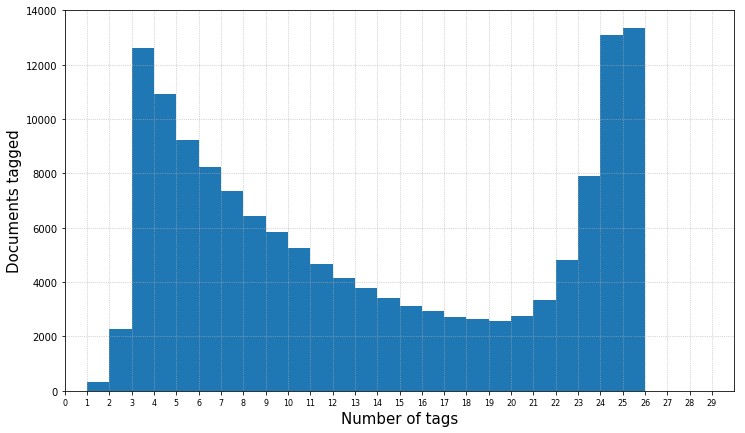
\includegraphics[width=\textwidth]{chapters/05_experiments/images/delicious_tag_per_resource.png}
    \caption{Distribution of the number of unique tags assigned to each document in the Delicious t-140 dataset (after pruning and preprocessing).}
    \label{fig:delicious_tag_doc_distr}
\end{figure}

\begin{figure}[!h]
    \centering
    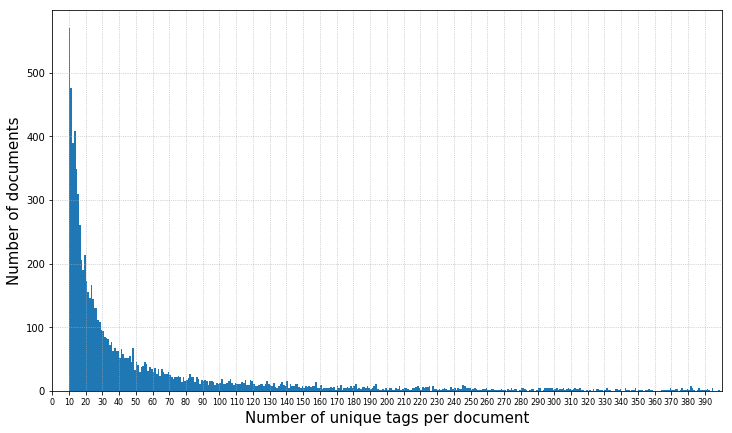
\includegraphics[width=\textwidth]{chapters/05_experiments/images/delicious_resource_per_tag.png}
    \caption{Distribution of the number of documents each tag was assigned to in the Delicious t-140 dataset (after pruning and preprocessing, not counting multiple assignments).}
    \label{fig:delicious_tag_doc_distr}
\end{figure}

\subsection{Dataset 2: Movielens 20M + IMDB Synopses}\label{subsec:dataset_2}

For our second dataset we chose one which, as previously explained, had different characteristics compared to the first dataset. We did this to verify whether (and to what extent) our methods and other methods perform in datasets which differ with respect to metrics such as average number of tags per document, total number of tags, etc.

Once again, we wanted to choose data from sources which have been often used in the literature. With that in mind, we chose to work with a MovieLens dataset and with movie synopsis data from the International Movie Database.

While it is true that combining both datasets yields another dataset which different from the first two, there are examples in the literature \citep{peralta_2007,kataria_2016} where these two datasets were combined.

\renewcommand{\arraystretch}{1.5}


\begin{table}[!h]
\centering
\caption{Dataset Statistics: MovieLens 20M + IMDB Synopses (after pruning and preprocessing)}
\begin{tabular}{|c|c{9}|}
\hline
\specialcell{Total number of Resources} & \,\,\, 6,710 &\\
\hline
\specialcell{Total number of unique tags} & \,\,\, 2,138 &\\
\hline
\specialcell{Average number of tags per resource} & \,\,\, 12.21 &\\
\hline
\specialcell{Minimum number of tags per resource} & \,\,\, 1 &\\
\hline
\specialcell{Maximum number of tags per resource} & \,\,\, 189 &\\
\hline
\specialcell{Average number of resources per tag} & \,\,\, 38.33 &\\
\hline
\specialcell{Minimum number of resources per tag} & \,\,\, 10 &\\
\hline
\specialcell{Maximum number of resources per tag} & \,\,\, 854 &\\
\hline
\end{tabular}
\label{tab:dataset_statistics_delicious}
\end{table}

\begin{figure}[!h]
    \centering
    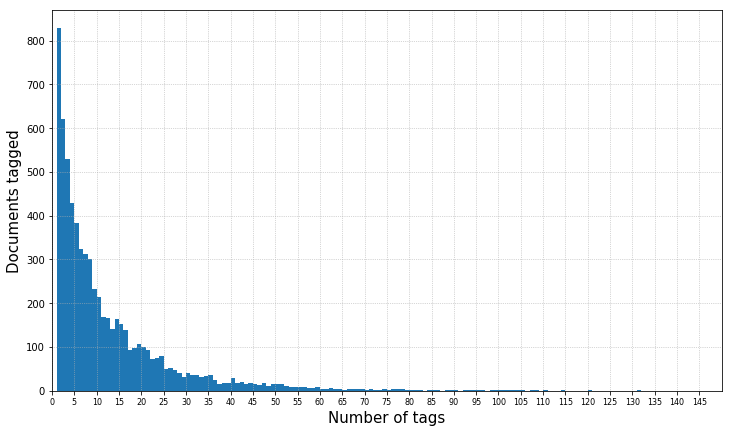
\includegraphics[width=\textwidth]{chapters/05_experiments/images/movielens_tags_per_resource.png}
    \caption{Distribution of the number of unique tags assigned to each document in the Movielens 20M + IMDB Synopses dataset (after pruning and preprocessing).}
    \label{fig:delicious_tag_doc_distr}
\end{figure}

\begin{figure}[!h]
    \centering
    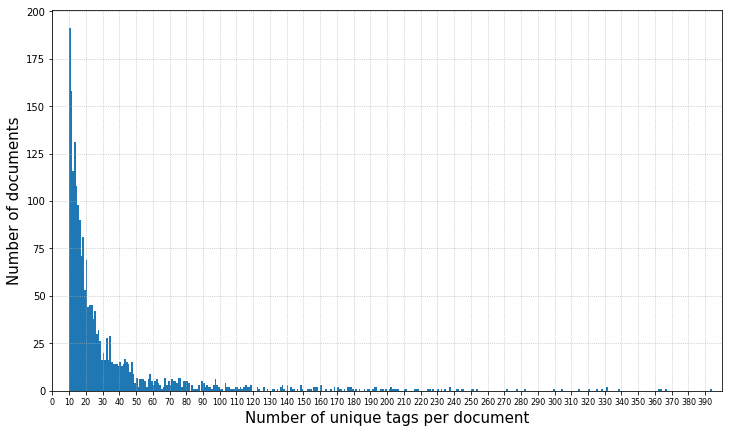
\includegraphics[width=\textwidth]{chapters/05_experiments/images/movielens_resources_per_tag.png}
    \caption{Distribution of the number of documents each tag was assigned to in the Movielens 20M + IMDB Synopses dataset (after pruning and preprocessing, not counting multiple assignments).}
    \label{fig:delicious_tag_doc_distr}
\end{figure}

\subsubsection{Construction and Preprocessing}

The first part of the dataset was obtained at https://grouplens.org/datasets/movielens/20m/. This download package includes a file with every tag assignment from \ednote{add earliest and latest date here}, for movies in the MovieLens website.

We preprocessed this dataset by normalizing all tags: lowercasing and removing special characters. In addition, we removed from the dataset all tags that occurred in less than 10 documents, following literature convention.

The download package includes a file that matches each MovieLens movie ID with the corresponding movie ID on the Internet Movie Database (IMDb) website \footnote{http://www.imdb.com/}. So, for each movie in the MovieLens dataset, its synopsis (when available) was manually scrapped from the IMDB website, using the \textit{Scrapy} \footnote{https://scrapy.org/} tool.

After crawling the website for the matching movie synopses, we saved the results and filtered out movies with non-english synopses.

\section{Experiment Outline}\label{section:experiment_outline}

In the following subsections, we will briefly explain the underlying reasons for the way we have setup our experiments.

\subsection{Method Selection}

These experiments are meant to address proposals \textbf{1)} (performance comparison of multiple tag-predictions approaches in two very different datasets) and \textbf{2)} (comparing the MIMLSVM tag prediction method using sparse and dense features). In order to have representative and non-biased experiments, we have chosen to use methods that were \textbf{a)} widely used in practice, \textbf{b)} different from other methods or \textbf{c)} both.

\subsection{Hyperparameter Tuning}

As is commonplace in most machine learning tasks, we have, for each experiment, tried a combination of hyperparameters for each method we have applied. We have used \textit{grid search}, probably the most common way to conduct hyperparameter search, to search for good configurations for the problems at hand. The actual search was done on a sample (generally 30\% of the full data) and the victor parameters used to train the model on the full datasets.

With respect to text-specific machine-learning, there is also the question of how to tune some feature extraction procedures. Once again, we have tried to emulate what has been done by other authors we have reviewed while also taking into account standard practice in the Natural Language Processing (NLP) field. We consider the two most important choices to be \textbf{a)} the number of words to use in BOW representation and \textbf{b)} the number of dimensions to use for word embeddings. We have conducted two simple comparisons to help us make appropriate choices for these parameters, taking into account both accuracy but also more practical matters such as training time and memory needed.

\begin{figure}[H]
    \begin{subfigure}{0.5\textwidth}
        \centering
    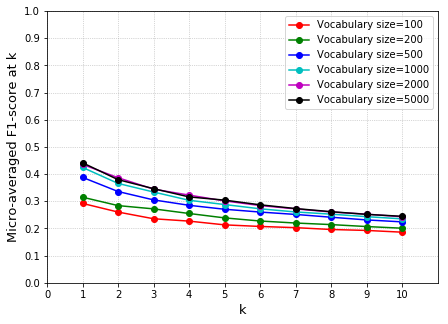
\includegraphics[width=0.8\textwidth]{chapters/05_experiments/images/comparison-vocabulary-size.png}
    \caption{Comparing performance using different vocabulary sizes (OvR SVM).}
    \label{fig:vocabulary_size_comparison}
    \end{subfigure}
    \begin{subfigure}{0.5\textwidth}
        \centering
    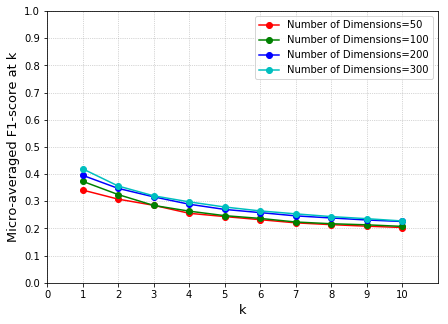
\includegraphics[width=0.8\textwidth]{chapters/05_experiments/images/comparison-number-of-dimensions.png}
    \caption{Comparing performance using different embedding dimensions. (OvR SVM)}
    \label{fig:embedding_dimension_comparison}
    \end{subfigure}
    \caption{Comparing choice of hyperparameters for feature extraction. Using Dataset 2 for illustrative purposes.}
\end{figure}

Based on the above tests, we have concluded that using a vocabulary with only 500 as the number of words and 100 as the embedding dimension represents a good trade-off between performance and training time and complexity. In other words, we consider these to be enough to enable comparing methods while not incurring long training times and extreme memory consumption.

\subsection{Metrics and Evaluation}

Problems with multi-label data (the type we have in this work) can be approached in one of two ways \citep{tsoumakas_2010,illig_etal_2011}: as \textbf{multi-label classification} or \textbf{label ranking}. The first type produces models that output a partition of labels (relevant/non-relevant) for each example. Conversely, label ranking implies training models that output an \textit{ordering} of labels for each instance. 

In this work, we have chosen to frame social tag prediction as a \textit{label ranking} problem. This follows standard practice in the literature but we also deem it more useful for real world tasks such as displaying a (finite) number of tag suggestions/predictions to users in an STS. In other words, the output of our classifiers will be a list of tags ranked in decreased order or relevance.

A wide variety of evaluation metrics\footnote{For extended commentary on ranking metrics see \cite{sokolova_and_napalme_2009} and \cite{kishida_2005}.} is used in label ranking. Among the many articles reviewed for this dissertation, we cite the following as the most commonly-used metrics in this domain.

\subsubsection{Average Precision and Mean Average Precision}

Average Precision (AP) is a widely-used\footnote{See \cite{buckley_vorhees_2000} for a comprehensive study.} metric to measure the result of a single list of ranked labels or a list of ranked documents (in an information retrieval setting).

In general terms, AP measures, up to a cutoff value $m$, the precision achieved considering all labels up to label $i$:  

\begin{equation}
AP_m =\frac{1}{m} \sum_{i=1}^{m} Precision@i \cdot \phi(i) \ ,
\end{equation}

where $Precision @i$ refers to the precision considering only the top $i$ labels; $\phi(t)$ is an indicator function whose value equals 1 if predicted label at rank $i$ is indeed a true label and 0 otherwise.

Now, when one wants to calculate AP over a whole dataset (as is out case), one can average AP over all documents for which we have predicted labels. This brings us to Mean Average Precision (MAP), which is calculated as follows:

\begin{equation}
MAP_m = \frac{1}{|D|}\sum_{d \in D} AP_m(d) \ ,
\end{equation}

where $D$ is the set of documents for which labels are to be predicted.

\subsubsection{Micro-Averaged F1 @k}

Another very commonly-used metric, and the one that we have chosen to work with, is \textbf{micro-averaged F1-score @k}

This measure was chosen due to the problem we wish to consider (namely, label ranking) and the way we want to average the results over a given dataset. In addition, this metric is commonly used in articles we have reviewed.

The F1-score (a particular case of the more general \textit{F-measure}, where $\beta$ equals 1) is widely used in information retrieval problems related to search or ranking of results; it is the harmonic mean of precision and recall, given by:

\begin{equation}
F_1 = 2 \cdot \frac{precision \cdot recall}{precision + recall} 
\end{equation}

which can be also written in terms of generic error metrics:

\begin{equation}
F_1 = \frac{2 \cdot true \ positive}{2 \cdot true \ positive + false \ negative + false \ positive} 
\end{equation}\\

With regards to \textit{micro-averaging}, it refers to the way we report results for the whole dataset, be it training or validation.

When \textit{macro-averaging} is used, equal weight is given to every class (label) in the dataset, which means that classes which occur only very rarely are given the same weight and very common classes when the full metrics over the dataset are calculated.

On the other hand, with \textit{micro-averaging}, the individual metrics (true positive, true negative, false positive and false negative) are aggregated over the whole dataset, which is preferable in cases (such as ours) where the dataset is highly unbalanced. \footnote{I.e. some labels appear much more often than others.}  

Finally, when metrics $@k$ are considered, it simply means that only the results up to the $k$-th position are taken into account when gathering the results:

\begin{equation}
F_1\ @k = \frac{2 \cdot true \ positive\ @k}{2 \cdot true \ positive\ @k + false \ negative\ @k + false \ positive\ @k} 
\end{equation}\\

This gives a more complete view of how the classifier works at different precision/recall levels, and can be easily visualized via graphical charts.

\subsection{Project Structure}

\subsubsection{Workflow}

{\color{red} TODO: Used jabref for keeping track of the referenced stuff}

{\color{red} TODO: Used jupyter notebook, for EDA, training and visualization.}

{\color{red} TODO: github for keeping track of changes and for collaboration}

{\color{red} TODO: sharelatex for writing this thesis}

\subsubsection{Frameworks and Libraries used}

{\color{red} TODO: jupyter}

{\color{red} TODO: python 3, numpy, scipy, sklearn, pandas, matplotlib}

{\color{red} TODO: spark, aws}

{\color{red} TODO: scrapy}

\subsubsection{Code layout}

{\color{red} TODO: Mention that the code is based off cookiecutter datascience, explain that it's supposed to help with reproducibility and help with keeping track of data versions. (need to cite them?)}

{\color{red} TODO: utils, helpers, etc}

{\color{red} TODO: throw in a graph }

\section{Experiments for Proposal 1}\label{section:experiment_part_1}

{\color{red} TODO: short introduction}

\subsection{TF-IDF weighted Bag-of-words Features, Binary Relevance + Linear SVM Classifier}

{\color{red} TODO: short introduction, add one or two examples of people using this.}

\subsubsection{Results on Dataset 1}

\begin{figure}[H]
    \centering
    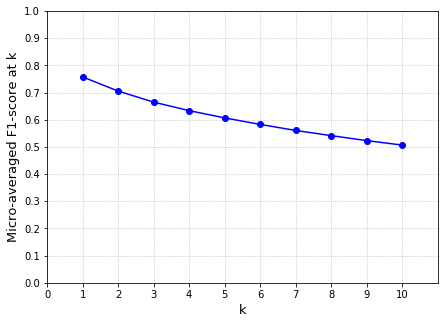
\includegraphics[width=7cm]{chapters/05_experiments/images/svm-tf-idf-delicious-20-frac.png}
    \caption{Results of applying Binary Relevance + Linear SVM with TF-IDF features on the Delicious t-140 Dataset}
    \label{fig:ovr_svm_movielens}
\end{figure}

\subsubsection{Results on Dataset 2}

\begin{figure}[H]
    \centering
    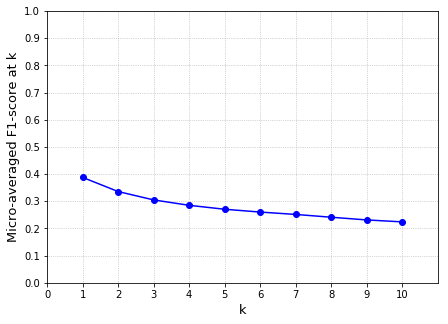
\includegraphics[width=7cm]{chapters/05_experiments/images/svm-tf-idf-movielens.png}
    \caption{Results of applying Binary Relevance + Linear SVM with TF-IDF features on the Movielens Dataset}
    \label{fig:ovr_svm_movielens}
\end{figure}

\subsubsection{Discussion}

\begin{figure}[H]
    \centering
    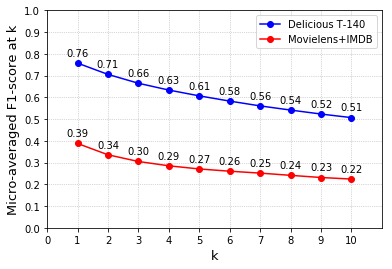
\includegraphics[width=7cm]{chapters/05_experiments/images/proposal-1-compared-ovr-svm-bow.png}}
    \caption{Compared results}
    \label{fig:compared_ovr_svm}
\end{figure}

As expected, the results in Dataset 1 were far better than those for Dataset 2, due to the differences in the tag distribution for both datasets.

It is interesting to note that the decrease in scores for Dataset 1 is somewhat more pronounced than in Dataset 2.

\subsection{TF-IDF weighted Bag-of-words Features, k-Nearest Neighbours Classifier}

The $k$-Nearest Neighbors is a very popular machine learning method that can be used both for classification and for regression. It consists in simply calculating the distances (assuming an $n$-dimensional representations) to every other instance, at \textit{inference time}\footnote{Methods such as $k$-NN are called \textit{lazy} methods because they need no training, as they defer all processing until actual inference is made.}. Then, each neighbor up to $k$ is treated as a source of information to help predict the class for the query instance. 

With respect to tag prediction, multiple (\cite{martinez_etal_2009,chidlovskii_2012,zhang_etal_2015,charte_etal_2015}\footnote{\cite{charte_etal_2015} have applied an approach very similar to ours, namely using multi-label $k$-NN to classify text into multiple tags, using TF-IDF representation. } to cite but a few) authors have applied some form of neighbor-based classifier to predicting tags for a query resource. 

In general, they proceed by finding nearest neighbors based on the resource's vector representation, as per the usual algorithm. Then, each neighbor's binary tag vector is added up and tags which are more commonly seen in the query instance's neighborhood are suggested.

Since we only want to use this method as a baseline, we implemented the most basic version thereof, namely simple, unweighted $k$-NN. Furthermore, we ran grid search over the method's hyperparameters, namely $k$, the number of neighbors to consider and also over the distance metric to use (cosine, euclidean, manhattan, etc).

\subsubsection{Results on dataset 1}

{\color{red} TODO}

\subsubsection{Results on Dataset 2}

\begin{figure}[H]
    \centering
    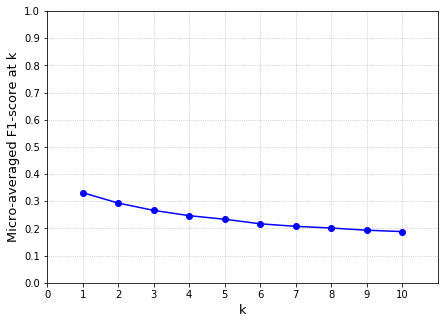
\includegraphics[width=7cm]{chapters/05_experiments/images/knn-tfidf-movielens.png}
    \caption{Applying $k$-NN on the Movielens Dataset, using TF-IDF weighted bag-of-words representation}
    \label{fig:knn__movielens}
\end{figure}

\subsubsection{Discussion}

Although the results were satisfactory, we would like to note that, surprisingly, using a \textit{weighted} variant did not increase performance on this task. In other words, weighing the contribution by the inverse of the distance to each neighbor did not increase the accuracy of the model.

\subsection{TF-IDF weighted Bag-of-words Features, Topic Distances}

In this approach, which has been suggested by \cite{choubey_2011},we first train a topic model on train set documents using Latent Dirichlet Allocation (LDA) (\cite{blei_etal_2003}). Then, at query time, we calculate the topic distribution for the query document and also the single most similar train set document, as measured by the Kullback-Leibler Divergence (KL-Divergence, \cite{kullback_leibler_1951}) between the topic distributions of the documents. Finally, the tags used in the found document are used as suggestions for the unlabelled query document.

\subsubsection{Results on dataset 1}

{\color{red} TODO}

\subsubsection{Results on Dataset 2}

\begin{figure}[H]
    \centering
    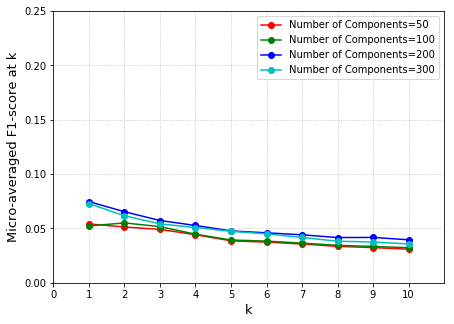
\includegraphics[width=7cm]{chapters/05_experiments/images/movielens-topic-distances.png}
    \caption{Applying Topic Distances on the Movielens Dataset, with varying values for the choice of LDA components}
    \label{fig:ovr_svm_movielens}
\end{figure}

\subsubsection{Discussion}

{\color{red} TODO mention results are around the same the original author got}

\subsection{TF-IDF weighted Bag-of-words Features, Topic Words}

In this approach, also suggested by \cite{choubey_2011}, one trains an LDA topic model on documents in the train set. At test time, the topic distribution for each query document is calculated with the trained model. Then, the most representative words \footnote{Only words that are in the actual tag vocabulary are used.} for the most representative topic are suggested as tags for the query document.

\subsubsection{Results on dataset 1}

{\color{red} TODO}

\subsubsection{Results on Dataset 2}

\begin{figure}[H]
    \centering
    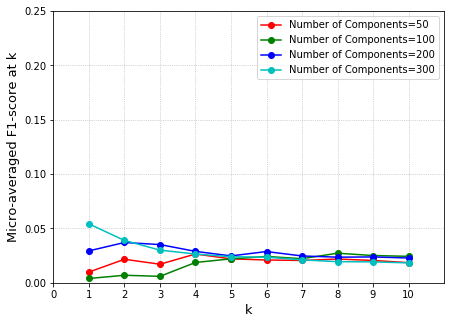
\includegraphics[width=7cm]{chapters/05_experiments/images/movielens-topic-words.png}
    \caption{Applying Topic Words on the Movielens Dataset, with varying values for the choice of LDA components}
    \label{fig:ovr_svm_movielens}
\end{figure}

\subsubsection{Discussion}

{\color{red} TODO mention results are around the same the original author got}

\subsection{LDA Topic Probabilities, k-nearest Neighbours Classifier}\label{sub:lda_topics}

Although Latent Dirichlet Allocation (LDA) \citep{blei_etal_2003} was originally created as a means to infer representative words for topics in corpora, it can be (and frequently is) used to extract features for documents. In fact, this approach was used and suggested in the original paper itself.

In other words, LDA can be used as a form of dimensionality reduction to reduce the size of feature vectors\footnote{Assuming an original bag-of-words representation without trimming the number of words used.} from $V$ to $k$, respectively the vocabulary size and the number of components in the LDA model.

Using these topic probabilities as features, we can then proceed onto classifying the documents using any classifier we wish. We have chose to use two classifier for this task: \textbf{a)} a simple $k$-nearest Neighours Classifier so as to enable comparison between using LDA features and using bag-of-words features and \textbf{b)} (in the next subsection) an SVM classifier, as suggested in the original LDA article.

\subsubsection{Results on dataset 1}

{\color{red} TODO}

\subsubsection{Results on Dataset 2}

\begin{figure}[H]
    \centering
    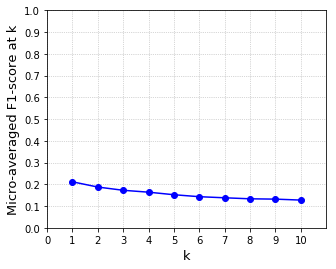
\includegraphics[width=7cm]{chapters/05_experiments/images/knn-lda-movielens.png}
    \caption{k-Nearest Neighbor classifier on the Movielens dataset, using LDA topic probabilities as features.}
    \label{fig:knn_lda_movielens}
\end{figure}

\subsubsection{Discussion}

\subsection{LDA Topic Probabilities, SVM classifier}

As mentioned on the previous subsection, we will compare results between both datasets using LDA as a simple dimensionality reduction step on top of TF-IDF weighted bag-of-words features. We will use an SVM classifier, as suggested in the original LDA paper by \cite{blei_etal_2003}.

\subsubsection{Results on dataset 1}

{\color{red} TODO}

\subsubsection{Results on Dataset 2}

\begin{figure}[H]
    \centering
    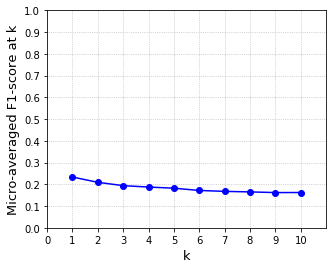
\includegraphics[width=7cm]{chapters/05_experiments/images/svm-lda-tf-idf-movielens.png}
    \caption{SVM classifier on the Movielens dataset, using LDA topic probabilities as features.}
    \label{fig:svm_lda_movielens}
\end{figure}

\subsubsection{Discussion}

{\color{red} TODO}

\subsection{Final Results and discussion}

{\color{red} TODO: as expected, results in dataset 1 were better but some were better, maybe because it's the way the features are represented.}

{\color{red} TODO: plot all experiments on a single graph to help people compare them}


\section{Experiments for Proposal 2}\label{section:experiment_part_2}

\textit{Multi-instance Learning}\footnote{Also called \textit{Multiple-instance} Learning} is a technique (the name was first coined by \cite{dietterich_etal_1997}), whereby a an  instance in a traditional supervised learning problem is split into multiple so-called \textit{bags}.

In other words, each individual sample in a dataset is represented not by a single feature vector but by a set thereof. For example, images may be represented as a bag of patches \citep{maron_ratan_98,andrews_etal_2003}, pharmacological drug molecules may be represented as a bag of configurations \citep{dietterich_etal_1997,andrews_etal_2003}.

\begin{figure}[H]
    \centering
    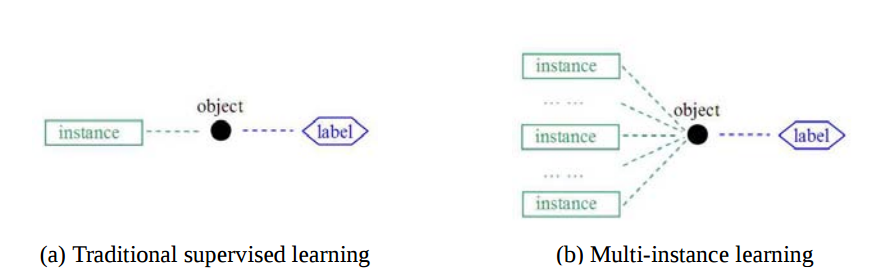
\includegraphics[width=0.8\textwidth]{chapters/05_experiments/images/miml1.png}
    \caption{Multi-instance learning works by representing a single example as multiple instances.}
    \label{fig:mimlsvm1}
\end{figure}

In 2006, \citeauthor{zhou_zhang_2006} have adapted the multi-instance learning paradigm into the multi-label setting, in the context of \textit{scene classification}. The main insight put forward by this work is that a multi-instance, multi-label (MIML) problem can be transformed into either \textbf{a)} a single-instance, multi-label task or \textbf{b)} a multi-instance, single-label task:

\begin{figure}[H]
    \centering
    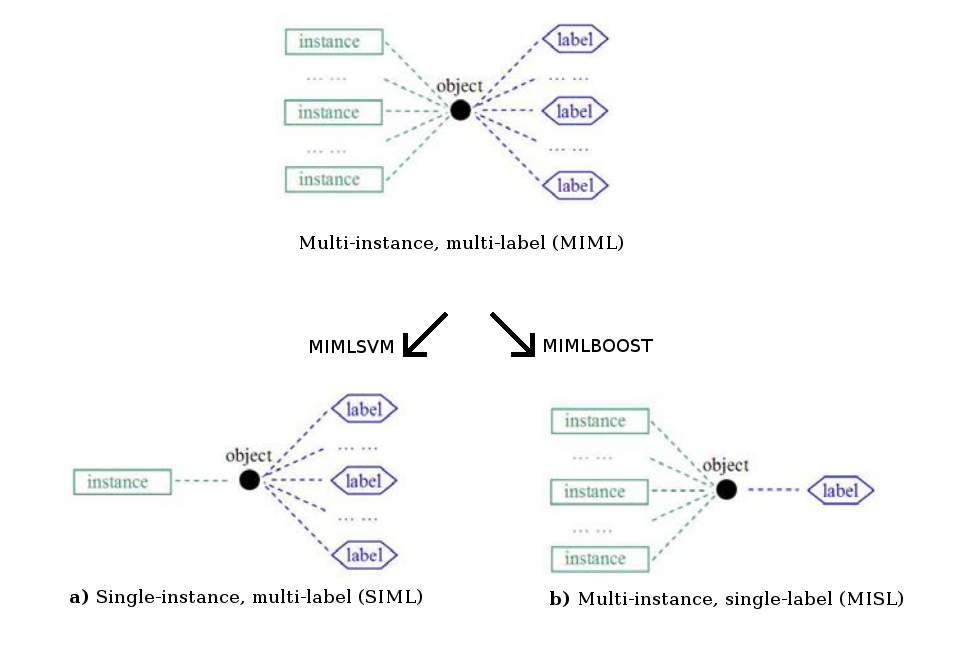
\includegraphics[width=\textwidth]{chapters/05_experiments/images/miml2.png}
    \caption{Original algorithm, devised by \cite{zhou_zhang_2006}, transforms an MIML problem into either a SIML or an MISL problem, using MIMLSVM and MIMLBOOST techniques, respectively.}
    \label{fig:mimlsvm1}
\end{figure}

In 2009, \citeauthor{shen_etal_2009} have applied multi-instance, multi-label (MIML) learning to the tag prediction problem. In particular, they have adapted the MIMLSVM algorithm from \cite{zhou_zhang_2006} to multi-label text classification.

The main idea here is that a single textual document may be split into multiple \textit{segments} via some kind of text segmentation algorithm. This makes it possible to view this problem as a multi-instance, multi-label (MIML) problem, where each segment represents one of many instances for a single document.

Each document is split into segments using a well-known text segmentation algorithm called \textit{TextTiling} (\cite{hearst_1994}). Then, these segments are vectorized into bag-of-words vectors. In order to turn the multiple segments into a single instance, the authors use \textit{k}-medoids clustering based on the Hausdorff distance (\cite{edgar_2008}). Finally, an SVM classifier\footnote{Configured so that it predicts a real-valued score for each tag instead of a binary prediction.} is applied on to the transformed dataset.\\ \\

\begin{algorithm}[H]
\LinesNotNumbered
\SetKwInOut{Input}{input}\SetKwInOut{Output}{output}
\Input{A set $D$ of text documents}
\Output{A trained SVM model to rank tags $y_d$ for every $d$ in $D$}
\BlankLine
 \textbf{Part I: Building a Single-Instance Dataset}
 
\ \ForEach{document $d$ in $D$}{
\BlankLine  
\tcp{split document into segments}\label{cmt}
$segments_d \leftarrow TextTiling(d)$    
  
  \BlankLine
  \BlankLine
  \tcp{transform each segment into a vector of features}\label{cmt} 
  $vectorizedSegments_d \leftarrow extractFeatures(segments_d)$ 
  
  \BlankLine
  \BlankLine
  \tcp{apply $k-$medoids clustering algorithm to the segments of $d$.}\label{cmt}
  \tcp{note that $features_d$ is now a single-instance vector}\label{cmt}
  \tcp{because Hausdorff Distance was used in clustering}\label{cmt}
  $features_d \leftarrow kMedoids( vectorizedSegments_d)$
  \BlankLine
  \BlankLine
  \tcp{this becomes a single row in the new $D'$ dataset}\label{cmt}
  $D'_d \leftarrow features_d$ 
 }
   \BlankLine
  \BlankLine
 \textbf{Part II: Training an SVM Classifier on $D'$}
 \caption{MIMLSVM applied to Tag Prediction \citep{shen_etal_2009} }
\ Train a $Ranked$ SVM algorithm on the transformed features in $D'$
\end{algorithm}

\hfill \break

The objective of the experiments in this section is to ascertain whether (if at all) the original results generalize to other kinds of features.

\subsection{MIMLSVM with IDF weighted Bag-of-words features}

{\color{red} TODO: this is the original implementation}

\subsubsection{Results on dataset 1}

{\color{red} TODO}

\subsubsection{Results on Dataset 2}

\begin{figure}[H]
    \centering
    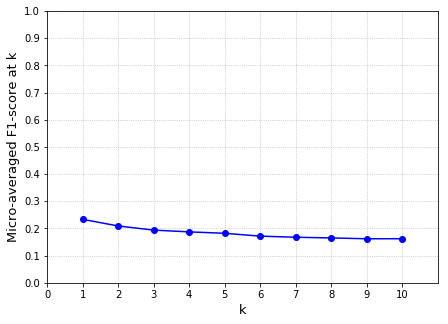
\includegraphics[width=7cm]{chapters/05_experiments/images/mimlsvm-tf-idf-movielens.png}
    \caption{MIMLSVM classifier applied on the Movielens dataset, using TF-IDF weighted bag-of-words features.}
    \label{fig:knn_lda_movielens}
\end{figure}

\subsubsection{Discussion}

{\color{red} TODO}

\subsection{MIMLSVM with LDA Topic Probabilities as Features}

Latent Dirichlet Allocation (LDA) \cite{blei_etal_2003} was originally thought of as an unsupervised method to learn the best way to infer latent topics for documents, based upon the distribution of words in them. 

As mentioned before in section \ref{sub:lda_topics}, the original LDA article itself suggests that topic probabilities be used as features to represent a document. This way, LDA can be thought of as a form of dimensionality reduction for documents, reducing the size of feature vectors from $V$, where $V$ is the size of the vocabulary to $D$, where $D$ is the number of components chosen when training the LDA model.

Each document is therefore represented as a feature vector of size $D$, where each $d_i \in D$ represents how much topic $i$ is present is a document, as per \cite{blei_etal_2003}. Since this vector is a dense vector, it serves out purpose of experimenting on using MIMLSVM on dense document representations.

\subsubsection{Results on dataset 1}

{\color{red} TODO}

\subsubsection{Results on Dataset 2}



\subsubsection{Discussion}

{\color{red} TODO}

\subsection{MIMLSVM with IDF-weighted Bag-of-embeddings Features}

\subsubsection{Results on dataset 1}

{\color{red} TODO}

\subsubsection{Results on Dataset 2}

\begin{figure}[H]
    \centering
    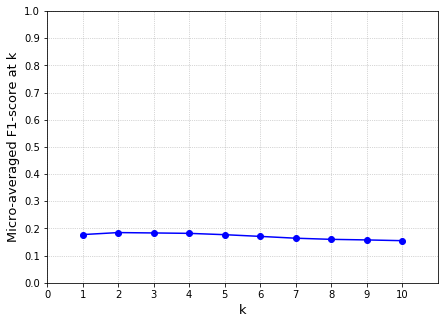
\includegraphics[width=7cm]{chapters/05_experiments/images/movielens-mimlsvm-embeddings.png}
    \caption{MIMLSVM classifier applied on the Movielens dataset, using TF-IDF weighted bag-of-embeddings features.}
    \label{fig:knn_lda_movielens}
\end{figure}

\subsubsection{Discussion}

\subsection{Final Results and discussion}

{\color{red} TODO: it looks like the results using dense features are worse.}

{\color{red} TODO: plot all experiments on a single graph to help people compare them}



    
	\chapter{Conclusion and Future Work}\label{chap: conclusion}


\section{Conclusion}


\section{Future Work}

\subsection{Alternative similarity metrics for clustering multi-instances}

The suggested approach uses the Hausdorff distance to calculate similarity between bags of instances, after a document has been split into segments. However, as suggested in the original article about scene classification \citep{zhou_zhang_2006}, Hausdorff distance is but one possible mapping to convert multiple bags into a single feature vector prior to performing clustering. 

Other distance metrics are available for comparing bags of vectors; \cite{huttenlocher_etal_1993} alone cite more than twenty variations that can be used under different conditions. Different metrics may yield different results, particularly when one considers not only sparse but also dense text representations.

\subsection{Alternative clustering algorithms}

While the $k$-medoids algorithm was used in the proposed approach, it remains to be seen whether other similar clustering algorithms could yield better results than those shown. In particular, similar, \textit{centroid-based} clustering algorithms include $k$-means clustering \citep{macqueen_1967}, $k$-medians clustering \citep{jain_dubes_1988} and $k$-means++ \citep{arthur_vassilvitskii_2007}.



	
	\backmatter
	\nocite{*}
	
	\bibliographystyle{coppe-plain}
	\bibliography{main}
	
	\appendix
	
	\include
	
	%\include{03_apendices//appenA}
\end{document}
